\documentclass[onecolumn, draftclsnofoot,10pt, compsoc]{IEEEtran}
\usepackage{graphicx}
\graphicspath{./Images/}
\usepackage{url}
\usepackage{setspace}
\usepackage{geometry}
\geometry{textheight=9.5in, textwidth=7in}

\usepackage[utf8]{inputenc}
\usepackage{array}
%\usepackage{wrapfig}
\usepackage{multirow}
\usepackage{tabularx}
\usepackage{multicol}
\usepackage{subcaption}

% 1. Fill in these details
\def \CapstoneTeamName{         BLAMO}
\def \CapstoneTeamNumber{               36}
\def \GroupMemberOne{                   James Trotter}
\def \GroupMemberTwo{                   Evan Amaya}
\def \GroupMemberThree{                 Sean Spink}
\def \GroupMemberFour{                  Alex Smith}
\def \CapstoneProjectName{              BLAMO}
\def \CapstoneSponsorCompany{   Oregon State University School of Civil and Construction Engineering}
\def \CapstoneSponsorPerson{            Matt Evans}

% 2. Uncomment the appropriate line below so that the document type works
\def \DocType{          %Problem Statement
                                %Requirements Document
                                %Technology Review
                                Winter End of Term Report
                                %Progress Report
                                }

\newcommand{\NameSigPair}[1]{\par
\makebox[2.75in][r]{#1} \hfil   \makebox[3.25in]{\makebox[2.25in]{\hrulefill} \hfill            \makebox[.75in]{\hrulefill}}
\par\vspace{-12pt} \textit{\tiny\noindent
\makebox[2.75in]{} \hfil                \makebox[3.25in]{\makebox[2.25in][r]{Signature} \hfill  \makebox[.75in][r]{Date}}}}
% 3. If the document is not to be signed, uncomment the RENEWcommand below
\renewcommand{\NameSigPair}[1]{#1}
\begin{document}
\begin{titlepage}
    \pagenumbering{gobble}
    \begin{singlespace}
%        
\includegraphics[height=4cm]{coe_v_spot1}
        \hfill
        % 4. If you have a logo, use this includegraphics command to put it on the coversheet.
        %\includegraphics[height=4cm]{CompanyLogo}   
        \par\vspace{.2in}
        \centering
        \scshape{
            \huge CS Capstone \DocType \par
            {\large\today}\par
            \vspace{.5in}
            \textbf{\Huge\CapstoneProjectName}\par
            \vfill
            {\large Prepared for}\par
            \Huge \CapstoneSponsorCompany\par
            \vspace{5pt}
            {\Large\NameSigPair{\CapstoneSponsorPerson}\par}
            {\large Prepared by }\par
Group\CapstoneTeamNumber\par
            % 5. comment out the line below this one if you do not wish to name your team
            \CapstoneTeamName\par
            \vspace{5pt}
            {\Large
                \NameSigPair{\GroupMemberOne}\par
                \NameSigPair{\GroupMemberTwo}\par
                \NameSigPair{\GroupMemberThree}\par
                \NameSigPair{\GroupMemberFour}\par
            }
            \vspace{20pt}
        }
        \begin{abstract}
        % 6. Fill in your abstract    
        This paper serves to give a major update and reflection of all the events and progress the BLAMO project has encountered over the winter term.We have been working on the project closely with our client  week by week in order to satisfy the needs and desires of the application. Also included is the current beta functionality goals that the project has accomplished, blockers that was met along the way, and what is currently left to do in the project before the code freeze in spring term.
        \end{abstract}
    \end{singlespace}
\end{titlepage}
\newpage
\pagenumbering{arabic}
\tableofcontents
% 7. uncomment this (if applicable). Consider adding a page break.
%\listoffigures
%\listoftables
\clearpage
\section{Project Recap}
Engineers and geological scientists currently are required to record all of their data on paper with a pencil when bore hole logging. After they would record the data on paper they would have to go back to their office and input the data into a proprietary software and get the desired output. Matt Evans from the school of Civil and Construction engineering at OSU has a need for a workflow that negates the extra cost and reliability on the proprietary software along with the flexibility of customization for their data logs.\par
This project is to improve the workflow previously mentioned by means of a mobile application. This application seeks out to be a fully fledged logging application that will assist and ease the engineers out in the field and allow them to focus on collecting accurate data.This application is also fully capable without any cell service or WiFi. The application itself has been developed using a new Flutter framework with dart as the language. It has been developed with the users at the front for the best possible user experience and usability out on the job with the assurance of no data loss and improved workflow.The end goal of the project is to have the complete workflow improved, local device save so the data is stored separate from the application and can be accessed at anytime outside of the app, and exporting the collected data as a CSV or PDF. 
\section{Current State of Project}
The current state of the project is that the application has all of its core components. It has all required fields and pages needed for a user to input all the data they will be recording out in the field. The application has an intuitive interface and navigation that partitions the different locations and associated documents so it protects the user from bad data input.The user can create new documents,tests,units, and convert their completed document to a PDF or CSV. There is also some elements in the user interface that are currently for development work only and will be removed when finished. 
\section{Work left to do}
As stated in the previous section all of the core workflows and integral parts of the application functions are all working properly. Since our product is going to be used by engineers out in an environment than none of us students are familiar with we still need to do tweaks to our user interface. This has been iterated on closely with feedback from our great client and he has been a great help with illustrating what works and what doesn't. Essentially the rest of the time period we have to work on this project will be tweaking elements of the interface here and there, taking more concentrated fine tuning feedback based on certain user tests. Since the start of implementation of this application we have done all of our testing through the emulator system that is provided by Android Studio and based all of our decisions off of that. Obviously, clicking with a mouse is a completely different feeling and understanding from a usability workflow. We will be putting our application onto phones and hopefully tablets to do more user testing with our client and potentially others. \par 
The other set of work that needs to be tackled is related to the usability and feedback the application gives to the user. Currently, the application has minimal feedback for when actions are completed, in progress, failed, or any other error that can occur. These errors are caught and printed out in the terminal for development purposes but need to be bubbled up to the user interface to notify the user. These features can also improve the aesthetic and clean look that our application is striving for. As a secondary stretch goal for extra polish we will be taking the advice we were given in our design review to look at the features of animation that Flutter provides.\par
Another portion of the project that was recently brought up was another layer of wrapping around document, and offering user compartmentalization of documents into overarching projects. To do this we will need to alter the file handler, and change how files are classified. The current standing of our app allows users to create documents, which would resemble a single borehole, but projects usually have multiple boreholes so we need a way to map boreholes to a project.
\section{Problems and Blockers}
Unfortunately, the biggest issue we have had with developing this project is Flutter. Flutter is the framework with dart being the language that we decided on to develop our application in. The reason that this decision had been made initially was to deliver the client wanting the application on both iOS and Android platforms.With that want in mind we flocked to Flutter because it had the capability of providing an avenue for developing on one code base and being able to deploy on iOS and Android respectively. This turned out to be the biggest blocker for our project due to a multitude of reasons. \par 
The most overlooked issue that we didn't asses properly in the designing phase was how new Flutter actually was. There have been multiple occasions where we run into a bug or some sort of issue with implementation of basic features and through digging find that there is no work around until the newer version comes out. We are talking Flutter being just about 2 years old and only just recently has it been expanding its features and fixing all the issues a programming language is released with. It has just been a learning experience all around with how difficult it actually is to implement newer technology. This has also been compounded by the fact that during this project a few of us have been taking the mobile development class offered here at OSU. This class has taught us skills about implementation and working in the application space that are useful and important. Unfortunately, the class has the skills taught in native Java for an android application and when we have tried to convert those skills into the Flutter space we have ran into a multitude of issues due to Flutter doing things just with a minuscule difference. \par 
Besides our trials and tribulations with Flutter we have been able to figure out solutions to most of the blockers that we have faced. The only feature blocker at the current moment is the ability to cloud save and email our files out of the application. In a traditional Android application you are able to open intents. An example of an intent is if you want to share a message or send a photo you just took to another person through email. This intent opens up your options for what application you want to use and it will navigate you to that application to send. However, in Flutter there is currently no way to implement this workflow of sharing files between applications other than providing plain text to another application. \par 
The lack of intents poses a major problem because we cannot use socket level programming of sending emails through SMTP because our application is not a verified google application and google authentication has strict security in place. The options that we sought out to work around this was to write custom code in native Android and share that way, offload the work onto a middle ware service such as Fire base, make a dedicated google email specifically for this application that does the email sending. The first option has major flaws due to writing custom code that will have to be written for Android and iOS, no guarantee that the mechanics of sending a Flutter activity to an Android activity is fully functional and not bug filled just like other features Flutter currently has. The second option has a huge upfront implementation requirement due to us having to integrate our application with this service and on top of that it does have fees associated with certain actions which result in the project costing annual money. The third option is workable but unfortunately leads to severe security holes and potential for bad actors to abuse the users of the application. The issue was brought up to our client and worked with him outlining the positives and negatives of the options I provided above. We decided as a collective that for the time being we will implement the feature as sharing plain text to the email application because the text can still be parsed and put into the appropriate locations as well as protecting the users.
\section{Code}
Some of the more interesting bits of code stem from the syntax of Flutter/Dart. Flutter works by containerizing widgets (A widget is a small U.I. module like a text-box or push button). The containerizing system of Flutter looks similar to how HTML would work with flex-boxes. For example, Figure 1 is a piece of our Document Overview page UI builder to further illustrate the point that for UI design Flutter is a breeze. However, while Uniformity is nice, in situations where we wanted to do something outside of the mold it was a lot more challenging. Flutter requires a lot more creativity with doing customized popups, or scroll boxes, especially with sizing.
\begin{figure}[!htb]
    \centering
    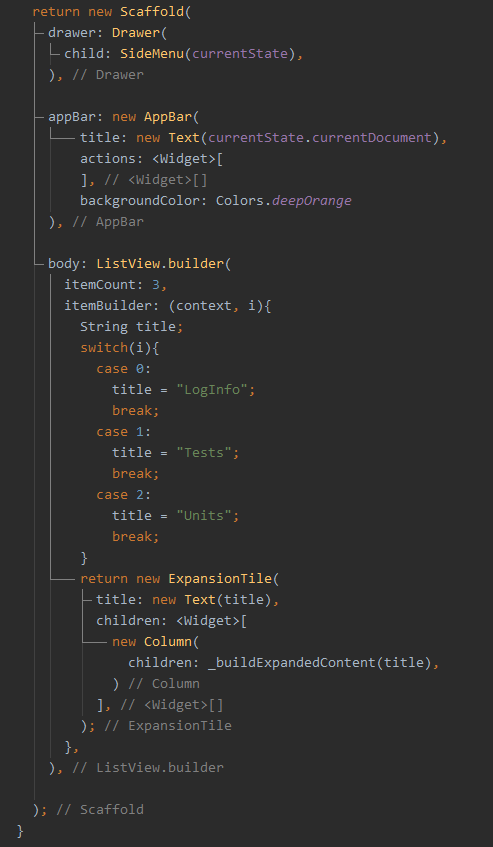
\includegraphics[scale=0.5]{Images/Capture.PNG}
    \label{Fig 1.}
    \caption{ Shows the code from the BLAMO Document Overview page, focusing on how scaffolds work}
\end{figure}
\par
After our experiences in the Android Development course offered here at OSU we moved to trying to do more layering, and as a result we produced ObjectHandler and FileHandler. The Object Handler takes care of Objectifying entry fields and either calling the FileHandler to save them, or Pull them for use. The whole purpose of the layering is to abstract away the Back-end heavy lifting from the U.I. allowing Flutters Front-End strengths to be coherent and truly shine, while using Dart for the back-end and not having too much of a mix of the two. After doing layering, a lot of our code was left looking more readable like for the Units Page (Fig 2.). In Figure 2 notice that the build function primarily deals with U.I. and mapping to external functions, as it should.
\begin{figure}[!htb]
    \centering
    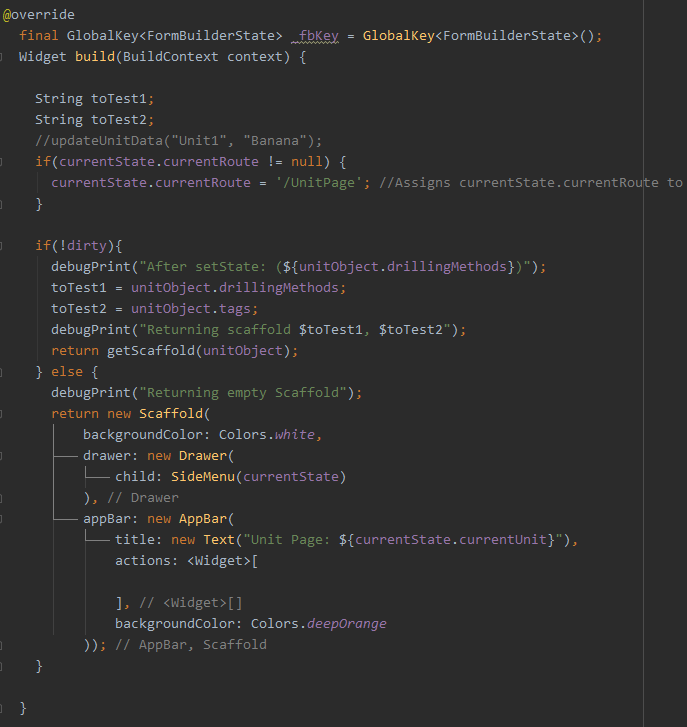
\includegraphics[scale=0.5]{Images/Capture2.PNG}
    \label{Fig 2.}
    \caption{ Shows the code from the BLAMO Unit page, focusing on how abstraction allowed UI building to focus on Flutter Key-Words}
\end{figure}
\par
In addition to helping readability for our code, the abstraction from the front-end helped to keep Async calls in order. When an Async function is called on a button press or on the opening of a page, Flutter/dart will call the Async function, and instead of having a call-back utilizes something called setState((values){todo()}) which essentially forces a redraw of a frame and to update the variables within that frame. As an example, our home page needs to populate with data that it pulls from a file, this requires an Async call, so initially the home page loads with an empty scaffold, but when the Async function calls setState() it updates the appropriate variables, and builds the appropriate scaffold. This is demonstrated in figures 3 and 4. Figure 3 shows the initial return logic when the page is opened, if the dirty bit (meaning data has not yet been returns) is set then it will return a page that includes a blank body, with a navigation bar (so if there is an error users can still navigate around). When the dirty bit is cleared, then setState is called, forcing build to be called again, and clearing the dirty bit. The application will then return a populated body that includes all of the Tests saved to the device.\newpage
\begin{figure}[!htb]
    \centering
    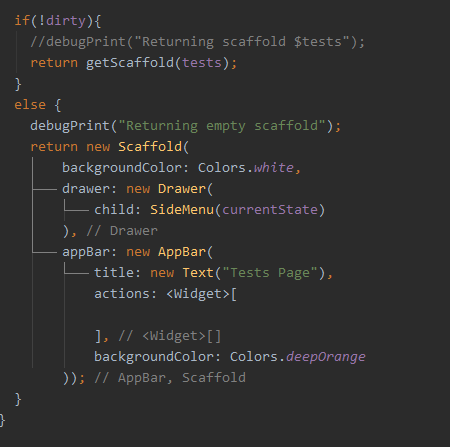
\includegraphics[scale=0.5]{Images/Capture3.PNG}
    \caption{ Shows the if logic for determining if data is populated yet for the tests page to build from}
\end{figure}
\begin{figure}[!htb]
    \centering
    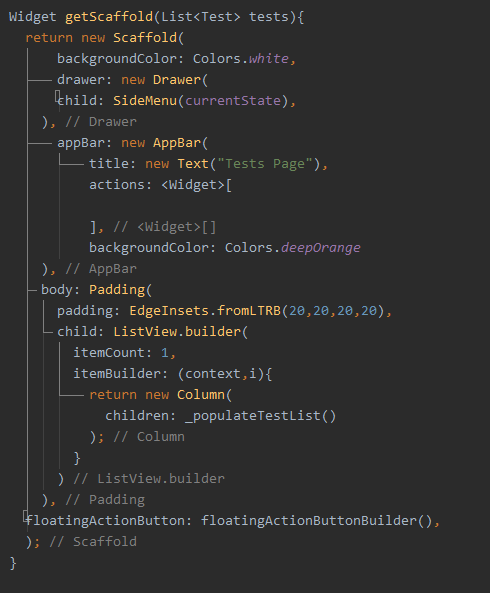
\includegraphics[scale=0.5]{Images/Capture4.PNG}
    \caption{ Demonstrates the populated scaffold building}
\end{figure}
\newpage

\section{Beta Functionality}
With beta functionality, our core functionality and foundation is implemented in terms of what we wanted to accomplish. There are still bugs and stretch goals, but if the project were to end today, the client would have baseline functionality. \par
As such, our application currently contains the functionality to enter information about soil and tests performed on the soil concurrently across drill sites and export data over email as needed by the user, which can be exported in either a CSV or PDF format. The application is usable without an internet connection, and would be able to be used in the field on a device by a logger to record data. On top of that the user has access to all data outside of the application if need be and manually modifying it with other applications. \par
Part of our work to get the application in a place where this functionality is usable, we had to clarify our navigation capability from our sidebar to better reflect our initial navigation plan, seen in the below diagrams.
This included wrapping all tests and units in respective landing pages, accessible from the navigation sidebar. The navigation sidebar's options change based on the application level the user is in.\par
Below are a number of screenshots demonstrating our expressed beta functionality and design. A walk through of the application and its processes can be found at the below link.

https://drive.google.com/open?id=1GPoqtwj0B1n1tVtLjC75ardJQRDZy3O-


\begin{figure}
\begin{subfigure}{.5\textwidth}
    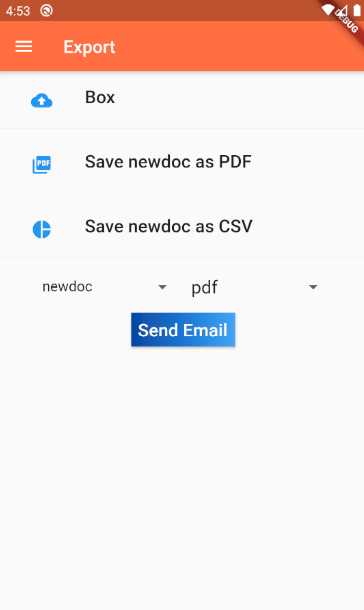
\includegraphics[scale=0.5]{Images/export.png}
    \label{Fig 6.}
    \caption{ The current export screen.}
\end{subfigure}
\begin{subfigure}{.5\textwidth}
    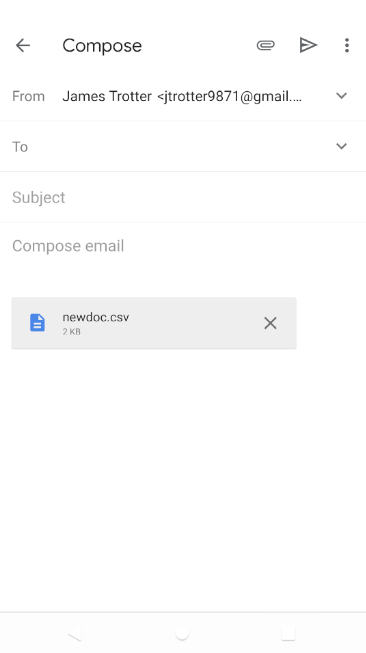
\includegraphics[scale=0.5]{Images/csvexport.png}
    \label{Fig 7.}
    \caption{ Emailing a csv file in-app.}
\end{subfigure}
\end{figure}
\begin{figure}
    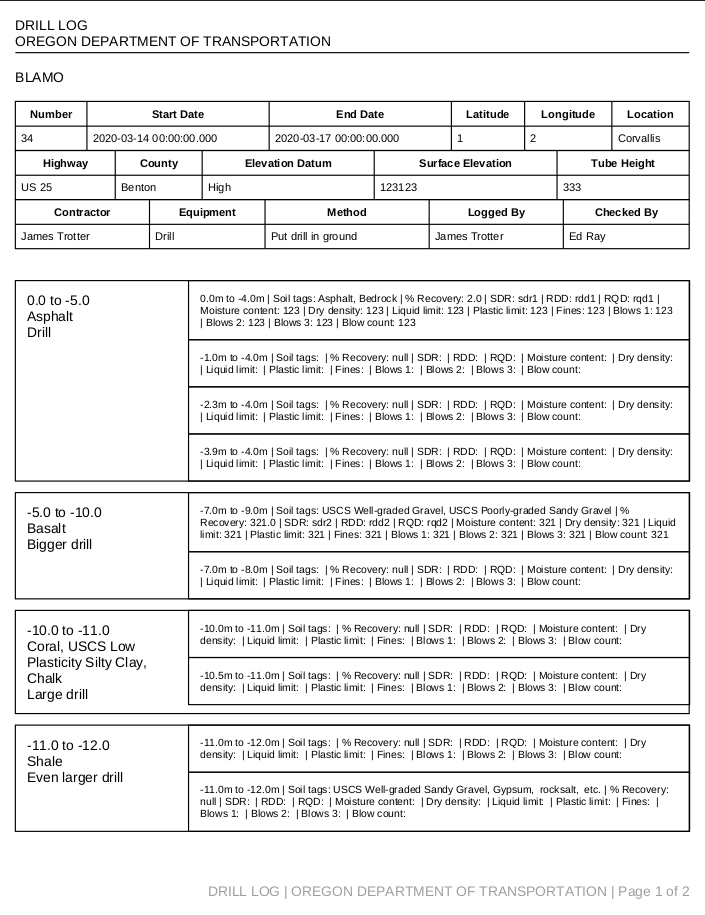
\includegraphics[scale=0.6]{Images/log1.png}
    \label{Fig 5.}
    \caption{ The current export PDF.}
\end{figure}
\begin{figure}
    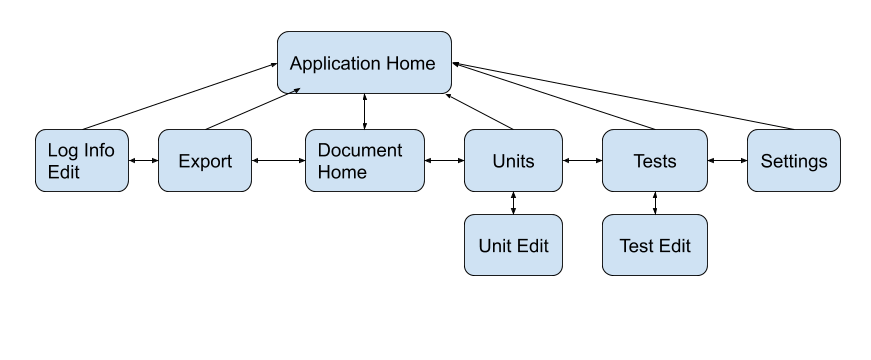
\includegraphics[scale=0.6]{Images/Navigation Diagram.png}
    \label{Fig 8.}
    \caption{ Application navigation map.}
\end{figure}
\begin{figure}
\begin{subfigure}{.5\textwidth}
    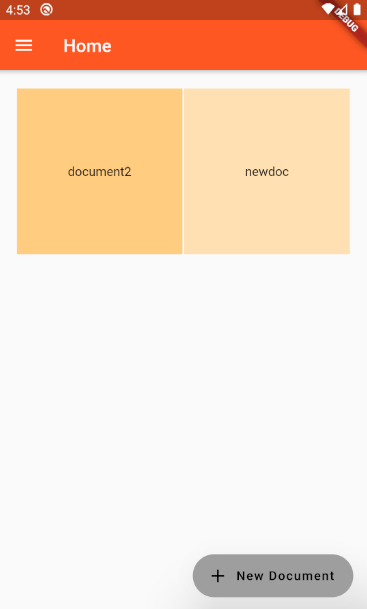
\includegraphics[scale=0.5]{Images/home.png}
    \label{Fig 9.}
    \caption{ The current application home screen.}
\end{subfigure}
\begin{subfigure}{.5\textwidth}
    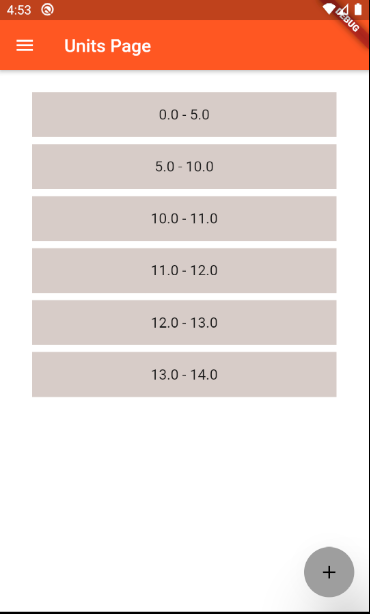
\includegraphics[scale=0.5]{Images/units_landing.png}
    \label{Fig 10.}
    \caption{ The units/tests landing page structure.}
\end{subfigure}
\end{figure}
\begin{figure}
\begin{subfigure}{.5\textwidth}
    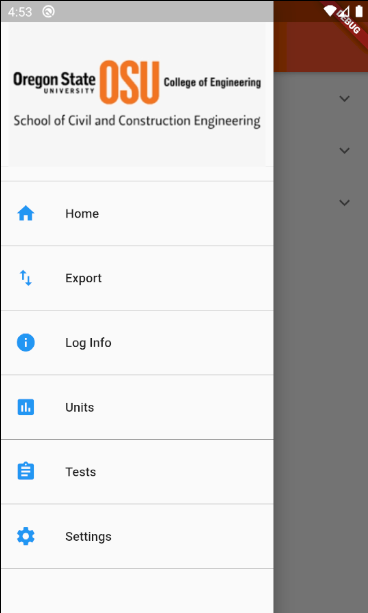
\includegraphics[scale=0.5]{Images/navbar_inapp.png}
    \label{Fig 11.}
    \caption{ The navbar from within a document.}
\end{subfigure}
\begin{subfigure}{.5\textwidth}
    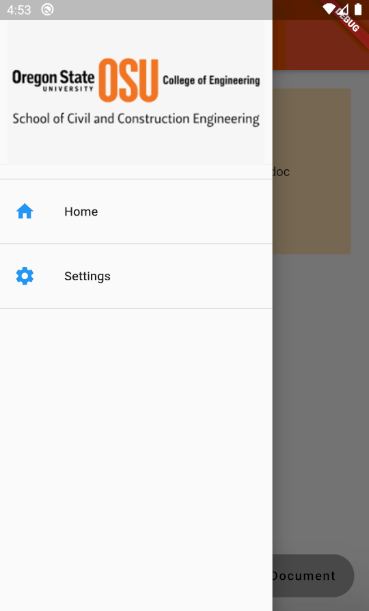
\includegraphics[scale=0.5]{Images/navbar_home.png}
    \label{Fig 12.}
    \caption{ The navbar from outside a document.}
\end{subfigure}
\end{figure}
\end{document}
                                                                                                                                                                                                                  92,9          Bot
